\section{Data Leakage}
This problem arises when some informaton in the validation set influences the training 
datase: the model isn't working with two independent sets. This lead to optimistic performance estimations, by which the model looks better than in reality.\\
\vspace{0.2cm}
This leakage might happen in a lot of situations, but they all have a common denominator: all has to be executed on the training data, not on the validation set, otherwise we have leakage.
\begin{itemize}
    \item scaling/standardization
    \item feature selection
    \item shrinkage/regularization
    \item PCA/feature extraction
    \item preprocessing
\end{itemize}
\begin{figure}[h]
    \centering
    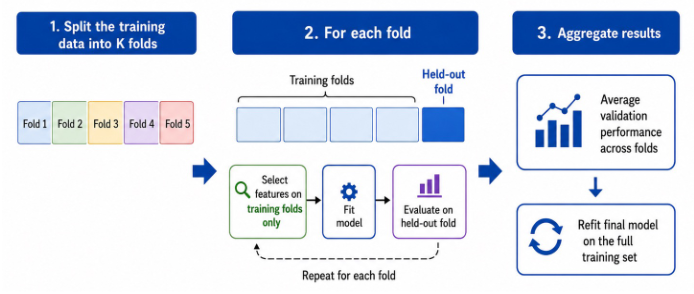
\includegraphics[width=0.75\linewidth]{img/data_leak_splitting.png}
    \caption{The splitting isn't something trivial.}
\end{figure}